\documentclass{article}
\usepackage{amsmath}
\usepackage{tikz}
\usetikzlibrary{calc}

\begin{document}

\begin{figure}[h]
    \centering
    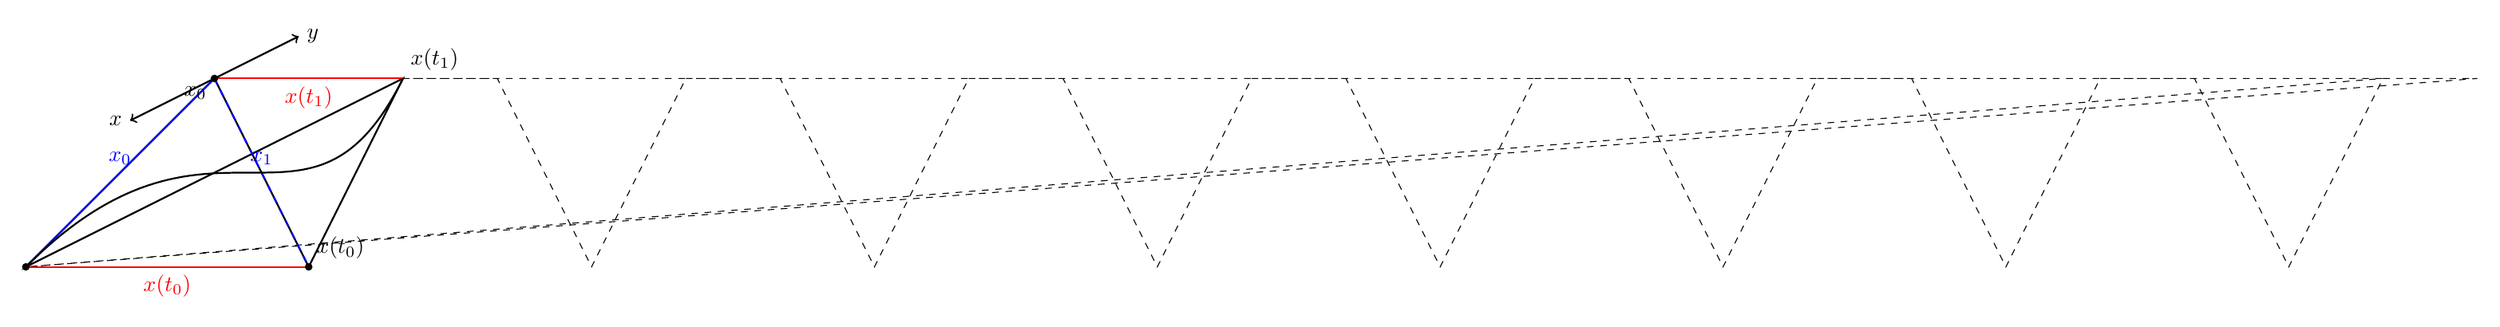
\begin{tikzpicture}[scale=1.5]
        % Define coordinates
        \coordinate (A) at (-1, -1);
        \coordinate (B) at (1, 1);
        \coordinate (C) at (2, -1);
        \coordinate (D) at (3, 1);
        \coordinate (E) at (4, 1);
        \coordinate (F) at (5, -1);
        \coordinate (G) at (6, 1);
        \coordinate (H) at (7, 1);
        \coordinate (I) at (8, -1);
        \coordinate (J) at (9, 1);
        \coordinate (K) at (10, 1);
        \coordinate (L) at (11, -1);
        \coordinate (M) at (12, 1);
        \coordinate (N) at (13, 1);
        \coordinate (O) at (14, -1);
        \coordinate (P) at (15, 1);
        \coordinate (Q) at (16, 1);
        \coordinate (R) at (17, -1);
        \coordinate (S) at (18, 1);
        \coordinate (T) at (19, 1);
        \coordinate (U) at (20, -1);
        \coordinate (V) at (21, 1);
        \coordinate (W) at (22, 1);
        \coordinate (X) at (23, -1);
        \coordinate (Y) at (24, 1);
        \coordinate (Z) at (25, 1);

        % Draw the tilted interval box
        \draw[thick] (A) -- (B) -- (C) -- (D) -- cycle;
        \draw[dashed] (D) -- (E) -- (F) -- (G) -- cycle;
        \draw[dashed] (G) -- (H) -- (I) -- (J) -- cycle;
        \draw[dashed] (J) -- (K) -- (L) -- (M) -- cycle;
        \draw[dashed] (M) -- (N) -- (O) -- (P) -- cycle;
        \draw[dashed] (P) -- (Q) -- (R) -- (S) -- cycle;
        \draw[dashed] (S) -- (T) -- (U) -- (V) -- cycle;
        \draw[dashed] (V) -- (W) -- (X) -- (Y) -- cycle;
        \draw[dashed] (Y) -- (Z) -- (A) -- cycle;

        % Draw the lines
        \draw[blue, thick] (A) -- (B) node[midway, above] {$x_0$};
        \draw[blue, dashed, thick] (B) -- (C) node[midway, above] {$x_1$};
        \draw[red, thick] (A) -- (C) node[midway, below] {$x(t_0)$};
        \draw[red, thick] (B) -- (D) node[midway, below] {$x(t_1)$};
        \draw[black, thick] (A) .. controls (B) and (C) .. (D);

        % Draw the points
        \filldraw[black] (A) circle (1pt);
        \filldraw[black] (B) circle (1pt);
        \filldraw[black] (C) circle (1pt);

        % Draw the axes
        \draw[->, thick] (B) -- ($(B)!1cm!90:(C)$) node[right] {$y$};
        \draw[->, thick] (B) -- ($(B)!1cm!-90:(C)$) node[left] {$x$};

        % Draw the labels
        \node at (B) [below left] {$x_0$};
        \node at (C) [above right] {$x(t_0)$};
        \node at (D) [above right] {$x(t_1)$};
    \end{tikzpicture}
    \caption{An illustration of the preconditioning in~\Cref{algo:preconditioning}. The point $x_0$ is an approximation of $x(t_0)$. The blue line represents the predictor step, and the blue dotted line represents the corrector step to get an approximation $x_1$ of $x(t_1)$. The line segment $s(t)$ connecting $x_0$ and $x_1$ is presented by the red line. The tilted interval box is centered at $s(t)$ at each $t\in [t_0,t_1]$ with the same radius.}
    \label{fig:preconditioning}
\end{figure}

\end{document}